\section{Results}

In order to get an operable demonstration of working composite video synthesis
some of the modules had to be bypassed. The digital interface was complete and
verified in simulation, however we did not have time to finish our video source,
Pong on the MSP430, so the digital interface was replaced by a simple verilog
module that fed the video generator a line that was white for the first half and
black for the second half. When displayed, the entire screen would be half white
and half black. Although not incredibly impressive, it did demonstrate that we
met our objective of generating a composite video signal.

\begin{figure} [H]
    \centering
    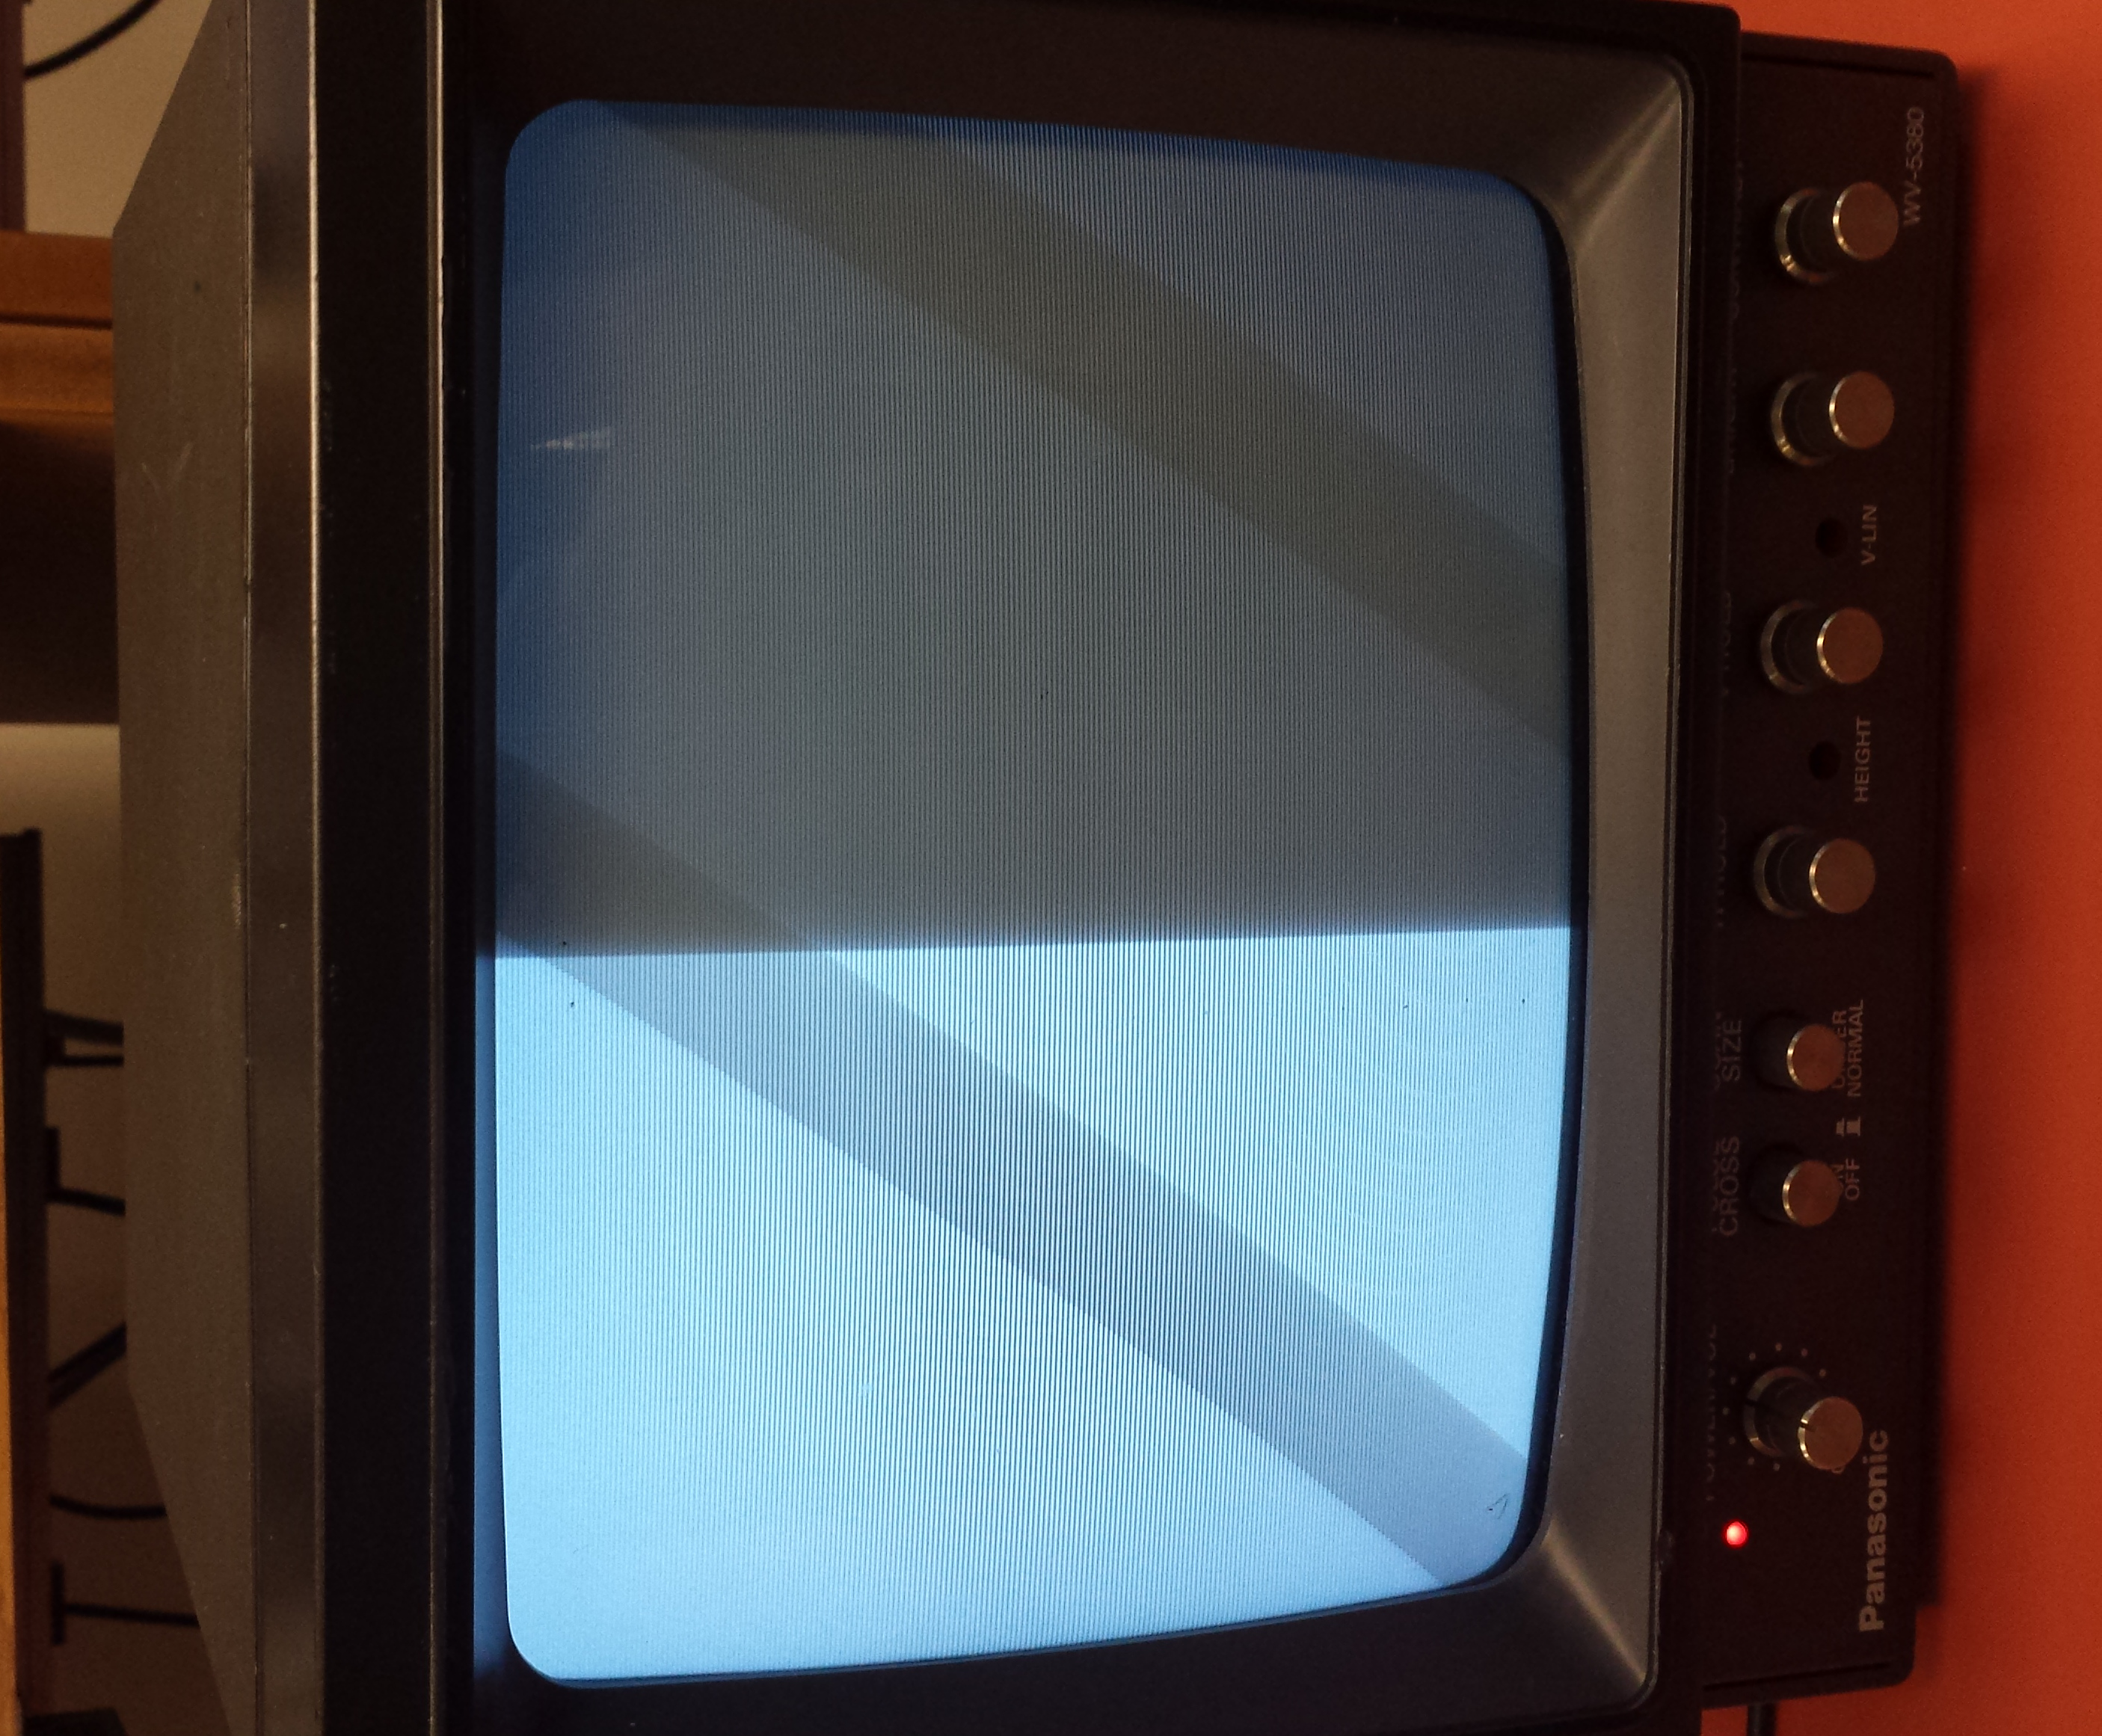
\includegraphics[scale=0.1, angle=270]{demoScreen.jpg}
    \caption{Demonstration Setup. Note: Grey diagonal bars are caused due to
    differences in the frame rate of the display and the shutter rate of the
    camera. The display is in fact half white and black.}
\end{figure}

Additionally, since we only had a black and white television, we were not able
to test our colour generation capability, however simulations of the module
output were successful. Here is the colour burst:

\begin{figure}[H]
    \centering
    \caption{Colour Burst}
\end{figure}

And here is the active video undergoing amplitude and phase modulation while
incrementing through the encoded colours.

\begin{figure}[H]
    \centering
    \caption{Phase and Amplitude Modulation}
\end{figure}
